\section{Methoden}

Zu Lösung der Aufgabenstellung wird die sogenannte YOLO (\textit{You Only Look Once}) Netzstruktur in Python unter Nutzung der Keras API implementiert. YOLO Netze zeichnen sich durch gute Detektionsergebnisse bei einer sehr hohen Trainings- und Klassifikationsperfomanz aus. So ist mithilfe des YOLO-Modells sogar auf vergleichsweise kostengünstiger Hardware eine Echtzeitschätzung der Bounding-Boxen von Objekten möglich \cite{Redmon2016}. 

\subsection{Lossberechnung und Intersection over Union}

Rezatofighi1 beschreibt die \textit{Intersection over Union} (IOU) als eine performante und präzise Möglichkeit den Loss bei der Objekterkennung zu bestimmen (s. Kap 2.2). Dabei wird die IOU aus dem Quotienten der sich überlappenden Fläche \textit{(Intersection / Overlap)} und der gemeinsam gebildeten Fläche (\textit{Union}) zweier Regionen berechnet: 
\begin{equation}\label{iou}
	IOU(y_{target},y_{pred})=\frac{y_{target} \cap y_{pred}}{y_{target} \cup y_{pred}}
\end{equation}
$y_{pred}$ steht hierbei für die geschätzte und $y_{target}$ für die reale Bounding-Box der Objekte. Die graphische Interpretation der Berechnung wird in Abbildung \ref{ioubild} deutlich. Zur Berechnung der jeweiligen Flächen wird der von Rezatofighil in \cite{Rezatofighi1902} beschriebene Algorithmus implementiert. Dort ist zusätzlich eine hier nicht genutzte Erweiterung zur \textit{Generalized-IOU} beschrieben.
\begin{figure}[!h]
  \centering
  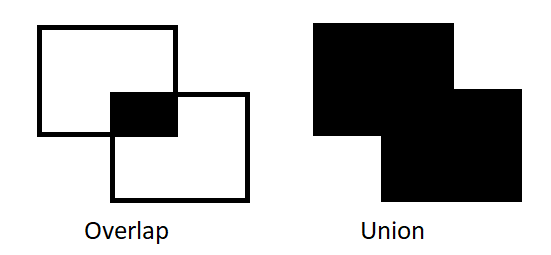
\includegraphics[width=8cm]{iou.png}
  \caption{Intersection over Union}
  \label{ioubild}
\end{figure} 
\FloatBarrier
Somit ergibt sich für den 2D-Fall als resultierende Loss-Funktion:
\begin{equation}\label{iouloss}
	L_{2D}= 1-IOU(y_{target},y_{pred})
\end{equation} 
Es ist darauf hinzuweisen, dass aufgrund der hohen Komplexität auf die Erweiterung der IOU Berechung für den 3D-Fall im Rahmen dieser Arbeit verzichtet wird. Im 3D-Fall wird der Loss lediglich über den in Kapitel 2.2. beschriebenen L2-Ansatz bestimmt. Möglich Ansätze für 3D-IOU Berechungen finden sich jedoch in \cite{Xu2019} und \cite{Mousavian1612}.

\subsection{Netzstruktur}

@Paul: hab das Paper gefunden, von dem unsere Netzstruktur inspiriert ist, da kannst du mal einen Blick rein werfen wenn du weitere infos brauchst: \cite{Redmon2016}

\subsection{Klassendiagramm}
Falls du bock drauf hast wäre es vlt noch sinnvoll grob das Klassendiagramm mit den Funktionen zu zeigen (aus python). Aber auf keinen Fall details. aber wenn du so schon genug hast reicht das auch ohne